\chapter*{Introduction}
\label{ch:Introduction}
This report illustrates development and findings of Group 2's project for
the course Text Analytics, Academic Year 2024-2025.

\section*{Team members and roles}


% copy-pasted from project proposal
\section*{Motivation and project goal}
Songs have the unique ability to engage people in ways that few other
mediums can match. While beats and melodies contribute to this impact,
it is often the lyrics that give songs their true emotional strength.
Lyrics serve as one of the main foundations of songs, playing
a crucial role in expressing feelings in many different ways.
Analyzing the emotional tone of song texts can give useful insights about individual mental states,
cultural trends, social issues and more.\\
% The main goal of this project is to perform emotion detection on stanzas of songs.
This emotional tone data can be useful
for many things, such as automatized playlist creation, or songs' organization,
offering an alternative to the more traditional genre-based classification.\\

The project's goal was to develop various Machine Learning models that perform this task.
Instead of detecting emotions for entire songs, the models assign emotion labels
to individual stanzas, to obtain a deeper understanding of
emotional fluctuations within the lyrics.
The emotional classification is based on Robert Plutchik's eight primary emotions
(shown in figure~\ref{fig:primary_emotions}),
offering a comprehensive range for representing diverse emotional states.\\
\begin{figure}[H]
    \centering
    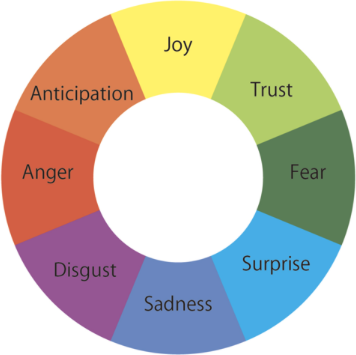
\includegraphics[scale= 0.5]{pictures/plutchik_primary_emotions.png}
    \caption{Plutchik's eight primary emotions}
    \label{fig:primary_emotions}
\end{figure}


Furthermore, we intend to compare different textual preprocessing and
Machine Learning models, in order to explore different possibilities and
evaluate their performances.

\section*{Chapter overview}
